\documentclass{report}
% Packages
\usepackage[utf8]{inputenc}
\usepackage{graphicx}
\usepackage{amsmath,amssymb}
\usepackage{hyperref}
\usepackage{geometry}
\usepackage{titlesec}
\usepackage{listings}
\usepackage{fancyhdr}
\usepackage{setspace}
\usepackage{csquotes}
\usepackage[T1]{fontenc}
\usepackage[style=authoryear-ibid,backend=biber]{biblatex}
\addbibresource{UoR_Masters_Project.biblatex}

% Page settings
\geometry{margin=1in}
\setlength{\parskip}{0.8em}
\setlength{\parindent}{0pt}
\doublespacing% Header and Footer
\pagestyle{fancy}
\fancyhf{}
\rhead{\thepage}
\lhead{ML-Powered Agile PM App}

% Title
\title{\textbf{An LLM-Powered Application for Agile Project Management}}
\author{Nithin Gandhi Simanand \\ Supervisor: Pat Parslow \\ MSc Data Science and Advanced Computing}
\date{\today}

\begin{document}

\maketitle

\tableofcontents

\newpage

% 1. Introduction
\chapter{Introduction}  % ~800 words
\section{Problem Statement and Motivation}

Enterprise-scale organisations routinely operate across a complex matrix of interdependent projects, movement across teams, and extensive resource portfolios. To maintain operational coherence and deliver value efficiently these firms typically rely on structured project management frameworks such as PRINCE2, PMBOK, or Agile-based hybrids. While such methodologies have demonstrated clear benefits in improving project visibility, governance, and stakeholder alignment, they remain susceptible to inherent inefficiencies. These stem largely from the rigidities of hierarchical communication, bureaucratic inertia, and the sheer scale of coordination required in large corporate environments \parencite{pricaEnhancingProjectEfficiency2025}.

Despite adherence to best practices, many firms continue to experience avoidable project delays, resource misallocation, and suboptimal decision-making cycles \parencite{mankinsTurningGreatStrategy2005}. A significant portion of these inefficiencies can be traced to human limitations in managing high-dimensional data, repetitive administrative tasks, and the cognitive overload associated with large-scale project orchestration. This presents a critical bottleneck: even with mature frameworks in place, enterprise project management often lacks the real-time adaptability and computational agility required to fully optimise performance at scale.

The emergence of Large Language Models (LLMs) and Machine Learning (ML) systems offers a transformative opportunity to address these structural inefficiencies. These technologies excel at pattern recognition, predictive analysis, and automating low-level cognitive functions, all attributes that align closely with the pain points of modern project management. By offloading repetitive, computation-heavy, and data-intensive components of project workflows to intelligent systems, organisations can enable human stakeholders to concentrate on strategic, creative, and high-context tasks where human judgment is irreplaceable.

However, due to the ever-growing importance of data protection, firms are increasingly hesitant to integrate cloud-based AI providers into their workflows. Concerns surrounding the ambiguity of how data is processed, where it is transmitted, and which datasets were used to train these models have created a significant barrier to adoption. While some organisations attempt to mitigate this risk by deploying locally hosted LLMs, these models typically function as open-ended chatbots. Consequently, the quality and relevance of their outputs are highly dependent on the user's ability to craft precise, context-aware prompts. Given the diversity in LLM interfaces, capabilities, and task specialization, employees without training in prompt engineering or a deep understanding of model behavior often struggle to extract meaningful value, effectively neutralising the potential gains these tools could offer.

This research is motivated by the need to bridge the gap between the theoretical capabilities of intelligent automation and their practical usability in real-world enterprise settings. The core problem lies not only in technical implementation, but also in aligning these systems with organisational workflows, ensuring security and compliance, and designing interfaces and processes that make advanced tools accessible to non-expert users. The goal is to explore how LLM- and ML-driven solutions can be securely, effectively, and intuitively integrated into large-scale project environments enabling genuine improvements in efficiency, responsiveness, and decision quality without compromising data integrity or overwhelming the workforce.


\section{Project Objectives}

There are four main objectives for this project:
\subsection{Develop a Multi-Dimensional Sprint Planner}
The first goal is to design an intelligent sprint planning system that automates the prioritisation and scheduling of project tasks. This planner considers multiple dynamic inputs, including team member availability, skill sets, task dependencies, organisational constraints, and regulatory and compliance related deadlines. The system is built to continuously ingest real-time updates, allowing it to refine project roadmaps dynamically as requirements shift. By embedding adaptive logic into the planner, the tool ensures that large-scale delivery remains aligned with strategic goals and operational timelines.
\subsection{Implement an Eisenhower Matrix-Based To-Do List Generator}
To enhance daily execution at the individual level, the system generates personalised task lists using the Eisenhower Matrix framework. This model categorises tasks based on urgency and importance, helping users focus on high-impact work while deferring or delegating less critical activities. These lists are continuously updated based on project context and user input, supporting focused, high-leverage productivity without manual task sorting.
\subsection{Integrate a Version Control System with LLM-Generated Commit Summaries}
The third objective is to ensure knowledge continuity and reduce the cognitive cost of context switching by embedding a version control system (VCS) into the platform. The VCS tracks project artefacts, decisions, and revisions, while an LLM generates automatic commit summaries that document key changes in clear, concise language. These summaries can be aggregated into progress reports, streamlining communication with internal stakeholders and external clients. Additionally, the system surfaces relevant historical context during task transitions, reducing ramp-up time and minimizing productivity losses across team handovers or project shifts.
\subsection{Ensure Secure, Containerised Local Deployment}
Finally, the project emphasises data security and deployment flexibility by containerizing the entire application for on-premise use. This architecture ensures that all data processing occurs within the organisation’s infrastructure, mitigating the risks associated with cloud-based AI platforms. The modular software design also supports plug-and-play integration of different LLMs for specialised tasks, allowing components to be updated independently without disrupting the user experience. By abstracting LLM interactions behind clearly defined workflows, the system eliminates the need for prompt engineering, making advanced AI capabilities accessible to non-technical users.

Testing for this project will focus on validating both functional performance and usability across the four core components. For the multi-dimensional sprint planner, tests will assess the accuracy and adaptability of task prioritization and scheduling in response to simulated changes in team availability, task dependencies, and deadlines. The Eisenhower Matrix task generator will be evaluated on its ability to categorise tasks correctly based on urgency and importance, as well as its impact on user focus and task completion rates.
The version control system and commit summarisation feature will be tested for robustness in tracking file changes, accuracy of LLM-generated summaries, and their usefulness in aiding project recall and progress reporting. Context-switching support will be assessed through user testing to measure reductions in ramp-up time when switching between tasks or projects.
Finally, the containerised deployment will be tested for security, performance, and reliability in an isolated enterprise environment. This includes ensuring data remains local, validating LLM module swap-ins’ do not disrupt functionality, and confirming that all features work without requiring prompt engineering. The specific details of the testing methodology will be outlined in the Methodology chapter with greater detail of the test cases available in Appendix \ref{app:TestLogs}.

% 2. Background & Literature Review
\chapter{Background and Literature Review}  % ~2000 words
\section{Project Management}

As this software project aims to assist enterprise-level organisations with project management, it is vital for it to interface with companies’ existing project management frameworks. This means ensuring that the workflow of the software does not in itself become a barrier to adoption, necessitating software-specific training and introducing new inefficiencies as a result.

In order to ascertain which framework would be the best to start working with, ‘Analysis and Comparison of Project Management Standards and Guides’ was reviewed \parencite{xueAnalysisComparisonProject}. Xue et al. sets out to analyse and compare three prominent PM references (PMBoK, ISO 21500, and ISO/IEC 29110) to assist project managers in making an informed choice, tailored to the scale of their project and its needs.

The motivation behind the study is grounded in the evolution of project management practices and the increasing need for clear guidance, especially in a landscape where projects vary vastly in size, complexity, and organisational structure. The paper begins by providing a historical context, illustrating that project management (PM) has been practised for millennia, and has continuously evolved with tools like Gantt charts, The Critical Path Method (CPM), Work Breakdown Structure (WBS), and Earned Value Management (EVM) becoming integral to contemporary PM. However, the variety of standards and guides, each designed with different target audiences, creates confusion for project managers, especially those unfamiliar with the subtle differences or lacking the time to conduct deep comparative analysis.

The analysis and comparison conducted directly responds to its problem statement by reducing the complexity around PM standard selection, thereby facilitating better adoption of PM practices tailored to project and organisational size. Furthermore, the paper’s discussion about the trend of large companies outsourcing to smaller suppliers underscores the growing importance of matching standards to organisational scale, especially as supply chains become more fragmented.

To gain a greater understanding, more research was conducted to identify the different project management methodologies used in industry. Reading ‘Analysis of the Available Project Management Methodologies’ \parencite{jovanovicAnalysisAvailableProject2018} once again highlighted that the effective implementation of project management methodologies remains a critical concern for organisations. Jovanovic et al. address a well-documented challenge in project management literature: the inadequacy of one-size-fits-all methodologies to accommodate the heterogeneous nature of projects across different sectors and scales.

The paper’s problem statement identifies a key gap: while numerous internationally recognised methodologies offer structured frameworks and processes, they often fail to consider the unique attributes of particular project types. This limitation is especially salient given the wide variance in project complexity, scope, and sector-specific needs. Agile methodologies emerge from the analysis as particularly well-suited to smaller, less complex projects, especially within the IT sector. Their iterative and flexible nature accommodates rapid change and uncertainty, addressing deficiencies in traditional methodologies, when applied to dynamic or fast-paced project environments. However, Xue et. al. find Agile’s applicability outside IT and similarly scoped projects remains limited.

The study’s synthesis underscores a critical implication: the suitability of any project management methodology is contingent on the interplay between project type, organisational culture, and management philosophy. This reinforces the necessity of moving beyond generalised processes towards methodologies that reflect the specific demands and contexts of project groups.  

The research alludes to future / further development of a modular system that can interface with a range of different project management processes, ensuring that the correct framework is used for the nature of each project and the team members involved whilst also ensuring that data flows smoothly between different projects following different management protocols.

A stand out point here is the claim made by Xue et. al. that the efficacy of Agile is limited. Serrador and Pinto explore the tangible impact of Agile methodologies on project success, offering empirical evidence to support the growing adoption of Agile practices in contemporary project management \parencite{serradorDoesAgileWork2015}. The core aim of the study is to assess whether the degree of Agile usage in a project is positively correlated with various dimensions of project success, namely overall success, efficiency (time and budget), and stakeholder satisfaction. This objective is positioned within a broader critique of the historically high failure rates of projects despite adherence to traditional methodologies, such as waterfall.

The paper is underpinned by data from 1,386 projects across various industries, providing a substantial empirical base. The methodology quantifies the extent of Agile implementation on a scale from 0% to 100% and measures its correlation with perceived project outcomes. The results reveal a statistically significant, though modest, positive relationship between Agile usage and project success, especially in terms of stakeholder satisfaction and overall success. While efficiency gains are less pronounced, they are still statistically valid. Notably, Agile practices did not reduce planning activity overall, rather, they redistributed it: less upfront, more iterative, suggesting a more adaptive planning model rather than an absence of structure.

Importantly, the study explores the moderation of variables such as project complexity, team experience, and clarity of project vision. Contrary to expectations, neither complexity nor experience significantly moderated the Agile-success relationship. However, projects with clearer visions saw enhanced benefits from Agile methods, indicating that the methodology’s success is not merely procedural but also context-dependent. The industry dimension adds further nuance: while Agile produced stronger positive effects in tech-oriented, healthcare, and service sectors, it had little to no effect in sectors with rigid planning requirements (e.g., construction, government). Serrador and Pinto provide empirical reinforcement for this project’s claim that Agile’s iterative and stakeholder-centric nature aligns more closely with the needs of modern, fast-moving projects than static, universalised methodologies.

However, the relatively low explanatory power (R² values around 0.02–0.15) underscores that Agile is not a panacea; other factors contribute significantly to project outcomes. The study advocates for a more sophisticated understanding of Agile, particularly its hybridisation with traditional methodologies; an area under explored yet reflective of current industry practice.

To gain a deeper understanding of the role of Agile,  key studies aiming to enhance project efficiency were reviewed. Prica et. al. offer a comprehensive examination of Agile Project Management (Agile PM) as a response to the limitations of traditional project management frameworks in complex, uncertain, and fast-paced environments. Central to this discourse is the critique of hierarchical, command-and-control paradigms, which are increasingly misaligned with the demands of knowledge-based, innovation-driven enterprise operations. This insight resonates directly with this project’s problem statement, which identifies structural inefficiencies rooted in bureaucratic rigidity and human cognitive limits as a primary obstacle in enterprise-scale project execution, despite the widespread adoption of established frameworks like PMBOK and PRINCE2 \parencite{pricaEnhancingProjectEfficiency2025}.

The literature traces the origins of Agile to the Agile Manifesto and Declaration of Interdependence, both of which prioritise adaptability, iterative delivery, and team autonomy over prescriptive process adherence. This decentralised model addresses a key challenge described in the problem statement: the human difficulty in managing high-dimensional, dynamic project data. The Agile emphasis on continuous feedback, sprint-based iterations, and role ownership provides a responsive structure that supports real-time adaptability, a core feature of the Multi-Dimensional Sprint Planner objective. These principles form the foundation for automating scheduling based on fluctuating variables, such as team availability and evolving compliance requirements.

The critique of traditional project theory reinforces the urgency for a paradigm shift. Their argument that models such as 'management-as-planning' and 'thermostat control'are insufficient aligns with this project's focus on replacing rigid planning with adaptive automation. Moreover, Williams et al.’s empirical findings, which show that PMBOK’s traditional frameworks hinder performance under uncertainty, support the necessity for LLM-augmented systems capable of pattern recognition and adaptive task reassignment. These findings validate the need for integrating ML systems that operate in fluid, decentralised contexts without relying on users to manually restructure plans or reports.

Coplien and Harrison’s pattern-based approach to Agile further complements the Eisenhower Matrix-based To-Do List Generator objective. They identify recurring behavioural and structural configurations that promote effective project execution. By learning from these patterns, intelligent systems can be trained to automate task prioritisation, not just based on importance or urgency, but also in relation to historical project behaviours and human productivity cycles, which is a layer of complexity that traditional planning tools overlook.

Finally, the literature also engages with Wysocki’s quadrant model, which categorises projects by goal clarity and solution certainty. This framework provides an analytical basis for determining when Agile, adaptive, or even extreme project management techniques are most suitable. The proposed system's ability to shift methodologies dynamically and autonomously mirrors this quadrant-based logic. Wysocki’s model offers useful heuristics for designing a sprint planner that fluidly adapts across the Eisenhower Matrix’s quadrants, ensuring that LLM-generated roadmaps remain contextually appropriate.

Much of the literature refers to ‘Agile Hybrids’: frameworks whose use compounds the benefits of the Agile methodology to increase its efficacy and applicability. In Agile Project Management with Scrum, Schwaber \parencite{schwaberAgileProjectManagement2004} draws a compelling analogy between Scrum and decentralised systems like road traffic or modern logistics, illustrating how simple rules empower independent agents to navigate complexity effectively. He positions Scrum as a response to the limitations of centralised planning in dynamic, uncertain environments. As projects grow in complexity, traditional command-and-control frameworks often fail while Scrum thrives by delegating decision-making to self-organising teams.

A key strength of Scrum, according to Schwaber, is its emphasis on short, iterative learning cycles that test complete business value propositions within 30-day sprints. This approach fosters continuous feedback, enabling developers to align more closely with shifting customer needs. Rather than pursuing rigid, front-loaded planning, Scrum adopts a test-and-learn philosophy aligned with Deming's cycle and other empirically driven improvement models. This aligns strongly with one of the key objectives of the project, using real time data to continuously improve and fine tune the sprint plan to ensure that the project remains on target even with shifting requirements and constraints.

Moreover, Scrum empowers teams to become ‘managers of their own fate.’ By entrusting workers with autonomy and purpose, Scrum taps into collective intelligence and real-time problem-solving. The model’s philosophical, managerial, and technical layers parallel the success of systems like Toyota's lean manufacturing, where trust, feedback, and long-term thinking underpin sustained performance.

In the paper ‘Agile Project Management: A Communicational Workflow Proposal’, the integration of Agile Project Management (APM) within Agile Manufacturing (AM) represents a paradigm shift toward adaptability, customer responsiveness, and continuous improvement in volatile production contexts. AM extends Agile principles beyond software into manufacturing, emphasising modularity, team autonomy, and fast response to dynamic customer demands \parencite{loiroAgileProjectManagement2019}. APM serves as the structural and procedural backbone of this model, guiding product development through iterative ‘momentums’ rather than rigid phases, from requirements analysis through to maintenance.

A central contribution of the paper is the proposed Agile team structure, comprising a Product Owner, Team Leader, and cross-functional Team Members, each playing dynamic roles throughout a product’s lifecycle. Effective communication, both within this team and with stakeholders, is deemed essential. The communication workflow, modeled in UML, facilitates the continuous integration of client feedback across key stages, aligning with core Agile values of responsiveness and customer-centricity.

However, the paper acknowledges significant barriers: cultural inertia, poor data literacy, and team readiness are cited as frequent obstacles to successful Agile transformation. While early results from implementation in a lighting manufacturing firm are inconclusive, the framework offers a promising, structured approach to embedding agility in non-software domains, provided organisations invest in education, communication, and role clarity.

A key takeaway from this paper is the proposed Agile Team structure, which has been modified and will be utilised in this project. Establishing a Team leader is important to ensure accountability and that the project has a strong vision; a factor that has already been established as vital to the success of the Agile framework \parencite{serradorDoesAgileWork2015}. Aligning the vision held by the leader and the business strategy in general with the project management framework is critical (as explored by \author{alsudiriAlignmentLargeProject2013}.) 

Prior research indicates that a significant proportion of projects fail to meet time, budget, and strategic objectives due to misalignment between PM processes and corporate strategy (Miller, 2002; Shenhar et al., 2007). While internal factors such as effective communication, executive support, leadership competence, and involvement of project managers in strategic development have been identified as pivotal to enhancing alignment (Eriksson, 2013), this study highlights equally important external factors, including government agencies, vendors, contractors, and site acquisition challenges, which substantially impact strategic implementation. The literature exposes a 'missing link'between business strategy and project plans, coined as 'project strategy'by Shenhar et al. (2007), underscoring the need for integrative frameworks that bridge this gap. Empirical findings reveal that companies often lack formal mechanisms to align and monitor the synergy between strategy and PM, adversely affecting project outcomes and business performance. This research contributes by applying stakeholder theory and strategic management processes to explain the complex interplay of internal and external influences on alignment. Ultimately, robust strategic alignment facilitates responsiveness to market dynamism and improves the realisation of business goals through effective project delivery.

In addition to this, a Cross Functional Team member system allows for greater exploitation of an individual’s skill-set, allowing for a level of flexibility that extends beyond task allocation based on a job title. However, this flexibility can lead to a lack of clarity as the number of tasks, subtasks and now the team members who are assigned to them, can vary greatly. 

The Agile methodology has a tool for improving continuous flow and tracking the progress of the subtasks of a project known as Kanban boards. In ‘ An Approach to Optimizing Kanban Board Workflow and Shortening the Project Management Plan’, Damij et. al. tackle the key challenge in Kanban implementation of how to effectively manage workflow on the Kanban board by finding the right balance among three critical parameters: replenishment value, work-in-progress (WIP) limits, and resource capacity \parencite{damijApproachOptimizingKanban2024}. The stated purpose is to go beyond the conventional focus on WIP limits alone and instead propose an approach that optimises the interplay between these factors to create a sustainable and efficient workflow. This purpose directly addresses the long-recognised problem that setting WIP limits in isolation often fails to produce consistent flow improvements, sometimes resulting in either idle team members or overloaded queues.

The paper’s motivation is rooted in the recent disruptions caused by the COVID-19 pandemic, which exposed the vulnerability of traditional working modes and highlighted the need for agile, adaptable workflows. Kanban is well-suited to meet this need, but practitioners struggle with applying its principles optimally, especially setting WIP limits that fit the actual capacity and demand of teams. The authors argue that sustainable flow depends not just on WIP limits but on harmonising those limits with replenishment (the rate new work is introduced) and the team’s resource capacity.

To validate this, the paper presents an empirical, simulation-based approach. By modelling the Kanban workflow and systematically varying replenishment rates, WIP limit combinations, and resource allocations, the authors generate data on key performance metrics such as lead time, queue lengths, and team utilization. This empirical method directly supports the paper’s objective to provide actionable insights rather than purely theoretical guidelines. The use of simulation here is clever:it allows 'what-if'experiments that would be impractical or disruptive in live projects and provides a controlled way to observe complex interactions among variables.

The results demonstrate that simply adjusting WIP limits without considering replenishment or resource capacity is insufficient for achieving continuous, smooth flow. For example, low WIP limits lead to team idleness, while overly high limits cause excessive queues and work overload, both of which degrade efficiency. The simulations identify optimal configurations where replenishment aligns with resource availability and WIP limits, producing a balanced system that minimises waiting times and maximises team utilisation. One key finding is that a replenishment value slightly above the number of resources in the initial stage yields the best performance, avoiding both bottlenecks and idle times.

This finding directly answers the paper’s problem statement by showing that Kanban workflow efficiency is not a simple function of WIP limits but a multi-dimensional optimisation problem. The authors’ approach reframes the challenge as one of finding an 'optimal relationship'or harmony among replenishment, WIP limits, and capacity, rather than trying to optimise any single factor in isolation. This aligns well with their project objective of developing a practical approach for Kanban teams to improve flow.

Moreover, the paper extends its contributions beyond theory, to practice. It suggests that managers who focus solely on maximizing resource utilisation without considering this balanced relationship risk creating dysfunctional workflows. By providing a systematic method, supported by simulation, to find the optimal parameters, the paper offers a tool that can reduce trial-and-error in Kanban board design, improve delivery predictability, and ultimately enhance team performance.

Finally, it is important to establish the difference that these project management frameworks will have to undergo as a result of the change in the industrial landscape to one where vast quantities of computational power is readily available. In the International Journal of Managing Projects in Business, \author{sonta-draczkowskaChallengesScalingAgile2024} argue that the accelerating complexity of project environments, driven by technological and social forces, has exposed the limitations of traditional models such as PMBOK and PRINCE2 \parencite{sonta-draczkowskaChallengesScalingAgile2024}. This argument reinforces the problem statement’s core premise: mature frameworks, despite their widespread use, are increasingly unable to cope with high-dimensionality, rapid change, and cognitive overload in enterprise-scale project environments.

The study highlights a fundamental misalignment between conventional project management practices and the nonlinear, emergent nature of digitally mediated work. Citing Brynjolfsson and McAfee, the authors frame digital disruption as an opportunity to reimagine how value is created and delivered, not just to merely automate existing processes. This is directly aligned with this project’s broader goal of integrating LLMs and ML systems not as auxiliary tools, but as foundational components for transforming task management, sprint planning, and decision cycles into adaptive, real-time systems.

The article outlines three stages of digital evolution in project environments: digitisation, digitalisation, and digital transformation, positioning LLM/ML integration clearly within the third stage. Digital transformation, as defined here, is not just about tools but about rethinking structures, roles, and value streams. This view supports the rationale for containerised deployment with plug-and-play LLM integration, where AI is not bolted onto legacy systems, but instead embedded into reengineered workflows that match how modern teams actually operate.

The discussion on human limitations, particularly the difficulty in anticipating interdependencies, managing unstructured data, and sustaining awareness across distributed teams, closely mirrors this project’s justification for developing a Multi-Dimensional Sprint Planner. The authors cite the rise of AI-assisted project management tools as a partial response, but stress that many existing tools still fail to close the cognitive gap due to poor interface design, lack of real-time feedback, and generic automation features. This directly maps to this project’s emphasis on removing the need for prompt engineering by abstracting LLM capabilities behind clearly defined workflows, allowing domain experts to engage with AI systems through intuitive interfaces.

Additionally, the paper’s critique of 'pseudo-agility'where organisations adopt Agile in form but not in function echoes the Eisenhower Matrix-based To-Do List Generator objective. It validates the need for personalisation and strategic alignment in task-level execution. By integrating LLMs to adaptively update task prioritisation based on real-time inputs (rather than static backlogs), the system described in the project objectives aims to support true agility, not just procedural mimicry.

The authors also point to an emerging challenge: the tension between speed and governance in large organisations. While Agile methods promote rapid iteration, enterprise environments are constrained by regulatory compliance and auditability. This justifies this project’s final objective of secure, containerised deployment, ensuring that LLMs operate within controlled environments where data sovereignty and traceability are preserved. It also supports the version control and LLM-generated commit summary features, which directly respond to the demand for transparency and historical accountability in AI-assisted workflows

Guan et. al.’s paper on Intelligent Virtual Assistants with LLM-based Process Automation aims to integrate the power of LLM processing with the primitive assistants found on mobile devices such as Amazon’s Alexa and Apple’s Siri. In their research they outline the main drawback of these assistants: the inability to 'carry out intricate multi-step procedures for their human users' \parencite{guanIntelligentVirtualAssistants2023}. They believe that utilising the natural language processing capabilities of LLMs and using them for process automation can allow these assistants to break down more abstract, high level requests and perform the individual steps in a manner that more replicates human-centric approaches.

The problem statement and the research conducted in this paper validates one of the problems that has been identified in this project: effective prompt engineering. In order to turn an abstract, high-level user request into an effective set of tasks to be completed, Guan et. al. takes a modular approach with modules for decomposing instructions, detecting interface elements and predicting future actions. By using \texttt{Alipay} as their target, they were able to demonstrate that their novel concept works, marking 'a major milestone in translating large language model research from controlled experimental settings into large-scale practical applications with tremendous reach and impact' \parencite{guanIntelligentVirtualAssistants2023}. This project is designed in such a way that there is no processing of abstract instructions, specifically to circumvent this issue but the study demonstrates the need for clear prompting and the benefits that can be gleaned when those are provided.

Integration of LLMs with human interaction is being explored in a range of industries with Chu et al. looking at the use of LLM agents in education. Their findings noted the widely appreciated benefits that LLMs can bring such as personalisation, collaboration and automation, all of which are also key advantages that translate into a project management context. However, they have also noted the ubiquitous issues of hallucinations, bias and fairness gaps. While education is contextually different, the parallels in privacy and deployment strongly reinforce the need for secure, bias-aware AI in enterprise project management. Given this, Chu et al.’s paper is a useful tool to critically evaluate how these ethical challenges express themselves in practice and how they can be neutralised. Chu et al find that 'self-correcting AI tutors'and 'teacher-in-the-loop' models are mitigations for hallucinations. This is reflective of the human in the loop workflow that is proposed for this project, with the authors’ research supporting that human AI feedback loops are essential for effective deployments.

Whilst there is no enterprise workflow integration evidence, this paper offers a comprehensive overview and forward-looking recommendations for challenges that transcend industry and are likely to be key hurdles in the PM context, as in both, the LLM would be a domain-specific agent, managing complex tasks and providing accurate plans. Chu et al explain that LLMs have been studied as tools to support students with Problem-Based Learning (PBL) wherein the pupils are tasked with real-world problem solving and project execution. However, ‘studies indicate that their effectiveness is limited by the absence of structured guidance frameworks that help educators and students seamlessly incorporate LLM agents into PBL workflows’. Many of the processes the AI supports overlap in both contexts, for example brainstorming, collaborative problem solving and project execution. While the need for a governing framework is implicit due to the size and context of projects in enterprise-level outfits, this is doubly reinforced when integrating LLMs into the workflow. This study reinforces the need for structural frameworks in the PM use case as well, as explored in this project’s problem statement which determined that orchestration (sprints, VCS, task automation) requires more than raw LLM capacity; it requires structural frameworks. The study shows that tasks considered only doable by humans, due to requiring nuanced judgement (e.g. both planning and teaching) can clearly be augmented with LLMs but with poor governance, the hurdles outweigh the benefits. This shows the need for clear auditability and strong Human-LLM integration. This also demonstrates the need for clear prompting to prevent issues like hallucinations and fully leverage the LLMs potential

White et al. explore prompt engineering techniques to control, refine and optimise LLM output, finding that 'prompt engineering is an increasingly important skill set needed to converse effectively with large language models (LLMs)' \parencite{whitePromptPatternCatalog2023}. Insights of the paper have informed this project, specifically its concrete techniques for and empirical insights into using prompt engineering to enhance LLM output. However, the paper focuses on surface-level interaction design and does not address deeper organisational integration or secure deployment, which approach has not been taken by this project. 

The authors show that effective prompting can reduce LLM hallucinations, improve reasoning and align the output with the user's actual intent, identifying zero-shot, few-shot, and chain-of-thought prompting as major paradigms for performance improvements. They provide empirical comparisons, showing performance gains when prompts are designed with contextual scaffolding and argue that prompt engineering is not a replacement for system design but a complementary control layer. This demonstrates that prompt engineering is a powerful enabler for this project’s objectives, but it requires embedding into a structured framework rather than being used ad hoc. This project’s structure imbibes this finding and capitalises on the edge provided by good prompt engineering by building it into the software, simultaneously eliminating the hurdle of ineffective prompts by non-technical users. The report supports Objectives one and two of this project since sprint planning and Eisenhower-style task classification require precise control over AI responses. The authors also argue that ‘prompt templates can be reused, but contextual grounding remains essential.' \parencite{whitePromptPatternCatalog2023} This aligns with this project’s requirements of a repeatable workflow in sprint planning and summarisation

Oluwagbade’s paper evaluating conversational AI in enhancing workplace inclusivity has also provided valuable insights to this project \parencite{oluwagbadeConversationalAINew2024}. The paper focuses on LLM-powered chatbots as mediators of communication in diverse workplaces and demonstrates that conversational AI can provide personalised support and also enhance collaboration across geographical and hierarchical boundaries, however the paper does acknowledge risks of bias in AI, privacy concerns, and the challenge of scalability. Conversational AI highlights the social and collaborative dimension of LLM deployment, reinforcing that inclusivity and bias-awareness must accompany technical optimisation. Oluwagbade describes the methods utilised: that of requirement analysis, fine-tuning, pilot testing, iterative refinement, and ethical oversight and proposes a framework for inclusive deployment, emphasising iterative feedback and monitoring, which are reflected in this project. The workplace context of this paper makes it highly relevant to enterprise use cases and as such means this paper has provided helpful insight into this project however, it does not address orchestration of complex tasks such as sprint management or VCS integration. 

Gaianu’s paper ‘On Premise Data Center vs Cloud’ compares On-Premise data centres with Cloud solutions, providing insights that aid in addressing this project’s problem statement regarding the trade-offs between self-managed infrastructure vs. outsourced cloud services.  The paper’s emphasis on evaluating Total Cost Ownership (TCO) over the long term when choosing between infrastructure solutions \parencite{gaianuPremiseDataCenter2023a}  informed the evaluation process for this project as it aligns with the objective to identify cost-effective and operationally efficient IT infrastructure options. Additionally, Shaji George’s approach \parencite{georgeCloudComedownUnderstanding2024}, underlined with the importance of realism when evaluating a solution and respecting the heterogeneity of business needs, was another important evaluative framework used. 
  
Cloud services allow for the dynamic scaling of resources and can adjust to meet business needs without intensive capital expenditure at the onset\parencite{gaianuPremiseDataCenter2023a}, \parencite{georgeCloudComedownUnderstanding2024}. Additionally, Thus, Cloud based infrastructure offers the benefit of offering operational agility and adaptability whilst also being cheaper than hosting resources locally. However, whilst requiring more investment in hardware, personnel and ongoing maintenance, On-Premises systems provide organisations with full control over infrastructure. Additionally, ‘if an organisation has high confidence in the capacity of internal IT resources and high confidence in their ability to deliver necessary results, then the On-Premise cost structure can be expected to save money over the longer term when compared to Cloud,’ parencite{gaianuPremiseDataCenter2023a} demonstrating that On-Premise infrastructure can still be the most cost-effective solution if internal expertise is strong. This finding reinforces the importance placed throughout this project of building an app that requires less training, information and maintenance to operate the software so that the benefits of On Premise solutions, which include data security and visibility, could be accessed without sacrificing cost-efficiency in this trade-off.

Gaianu’s paper also highlights  how different stakeholders approach both systems. Vendors favour Cloud subscriptions for predictable revenue however, whilst, On-Premise data centers still maintain a significant share due to regulatory, security and compliance needs. Although there are potential vendor biases in favour of Cloud systems, the comparative regulatory ease and ease of compliance offered by On-Premise solutions remains a key advantage, when viewed through the lens of key grounding principles of this project, namely ease of integration and sustained use and emphasis on data security. 

The research of Shaji George validates this point further, explaining that notable cloud breaches, for example at Capital One and Twilio, underscore a growing apprehension for storing data externally \parencite{georgeCloudComedownUnderstanding2024}. When coupled with the outages that have been experienced across major providers such as Azure and Oracle, as well as the dominance of the market by ‘The Big Three’ which restrict innovation and user choice surrounding price, service and ecosystems, Cloud services can be seen to increase user dependence on external providers, decrease choice and so, in both cases increase vulnerability. As a result of this, there is a rising trend of ‘Cloud Exit’ , with firms moving back to On-Premise systems or hybrid systems. A key reason for this is also cost management, with 93\% of leaders citing unchecked spending as a motivator, as ‘cloud savings didn’t automatically pass to users’ (\parencite{georgeCloudComedownUnderstanding2024} p5). 

However, it is important to address that Cloud solutions are not being disregarded in their entirety, with many businesses adopting hybrid approaches to avail themselves of the benefits of both approaches, something that is beyond the scope of this project but an area for possible further development. At this stage, On-Premise solutions have been chosen as they offer ‘enhanced oversight, security, compliance, costs savings and performance’ \parencite{georgeCloudComedownUnderstanding2024} (p.8) and thus, align best with the strategic goals of this project. Additionally, given that 65\% of IT decision makers plan to move the majority of cloud-hosted data within 12 months’ \parencite{georgeCloudComedownUnderstanding2024}, it indicates that the solution best suited to the near future, which also offers most ROI within the scope of this project, is On-Premise infrastructure. 


Spinellis argues ‘if you or your project isn’t using a VCS, adopting one might well be the single most important tooling improvement you can undertake’\parencite{spinellisVersionControlSystems2005}. Many of the benefits they outline have informed this project as they facilitate its key objectives. Firstly, VCS prevents developers from overwriting each other’s work, automatically merging changes or warning about conflicts. This feature is particularly useful to this project as it supports the key goals of collaborative efficiency and reduction of errors in multi-developer environments, necessary in a PM context. Additionally, every commit generates a new version, with logs indicating who changed which lines which enables historical tracking and accountability, facilitating this project’s objective of maintaining robust code provenance, useful in auditing or debugging complex systems. Moreover, VCS allows splitting work into branches, labeling releases, and mining repository data for productivity analysis which supports this project’s goals of structured release management, version traceability, and performance monitoring. 

Many projects run inefficiently without a version control system, even though editors and compilers are universally adopted, highlighting the importance of structured development practices in this project’s objective of improving software quality and maintainability. Additionally, from the perspective of a cost-benefit, a throughline for this project, the research shows that implementing a VCS aligns with this project’s objective of improving development workflows feasibly without major financial investment as VCS implementation does not need to be expensive, with free open-source systems like CVS or RCS being reliable for large projects.

Docker containers are OS-level virtualisation tools that focus on running applications rather than emulating hardware in turn reducing overhead and improving scalability \parencite{vaseAdvantagesDocker2015} , which supports this project’s objectives of deploying efficient, lightweight systems and optimising resource utilisation. Additionally, Docker containers offer ‘portability, delivery, scalability, speed and density’ \parencite{vaseAdvantagesDocker2015}, each offering increasing usability and decreasing operational hurdles faced by developers and system operators or decreasing the time taken for each task; directly supporting the project objective of improving deployment efficiency and developer productivity. Moreover, containers launch in sub-second times and allow high-density deployments on a single physical host \parencite{vaseAdvantagesDocker2015} which facilitates the improvement of system performance and rapid deployment, especially in cloud or enterprise environments, thus supporting this project in the realisation of these objectives.

‘One of the biggest problems removed is the “dependency hell” as containers contain all the needed dependencies and therefore properly executed and built containers are guaranteed to work in every other Docker instance’ \parencite{vaseAdvantagesDocker2015}. The ‘dependency hell’ problem Docker solves for supports this project’s problem statement regarding the need for reliable deployment pipelines and reducing environment-related failures and its use facilitates this goal. Defense-in-depth and least-privilege principles are emphasised improving system security. Additionally, properly configured Docker containers provide additional isolation and control, both features address this project’s objectives concerning secure deployment practices and safeguarding enterprise applications.

Dmytryshyn’s study on the Eisenhower Matrix emphasises that time is a limited and valuable asset, and managing it effectively directly impacts productivity \parencite{dmytryshynProposalEffectiveTime2022}.This analysis mirrors the principles underpinning this project and validates its objectives of optimising workflows, efficiency, and task prioritisation in enterprise. The paper introduces an algorithm to systematically identify and resolve time management problems, including procrastination, inability to achieve goals, and lack of time with activities including time tracking, bottleneck identification, evaluation, and repeating the study to improve planning and execution.  Additionally, tasks are classified by urgency and importance, guiding prioritization and delegation, and non-essential tasks (‘non-urgent and non-important’ tasks) are minimized. The success of this algorithm in increasing productivity supports the influence of the Eisenhower Matrix in informing project design in workflow management as it allows for adjustment based on individual characteristics and circumstances, supporting this project’s objectives for flexible, user-focused systems that adapt to different environments or user needs. Additionally, it provides practical evidence in favour of creating structured, repeatable processes that improve efficiency, which could integrate with digital tools or task automation and facilitate the objectives of  monitoring effectiveness and iteratively improving operational performance.


% 3. Methodology
\chapter{Methodology}  % ~1500 words

From the outset, the objectives were clear: to create a project management tool that integrated the power of large language models (LLMs) while maintaining security, locality, and accountability. Existing solutions in the market tended to sacrifice these values in exchange for convenience, relying on cloud platforms that expose users to surveillance, data harvesting, and opaque decision-making. The aim of this project was to show that another path was possible.
Yet the path was not straightforward. The final system—a lightweight Python application with a QML interface—was the result of iteration, reconsideration, and adaptation. Early versions of the project looked very different. At first, the system was conceived as a web application, powered by a centralised server that would process requests and host LLM modules. This design was motivated by performance. By placing the model on a server, more powerful language models could be deployed, models that would be too resource-intensive for individual user machines. The web interface, meanwhile, would give users familiar access through their browsers, requiring no installation and simplifying the experience.
The concept was attractive in theory. It promised scalability, flexibility, and the possibility of stronger AI performance. However, it soon became apparent that this approach was not viable within the scope of the project. Building and maintaining a server-side architecture, with user authentication, task persistence, and model hosting, would require a skillset in web frameworks and frontend languages such as React. Lacking prior experience with these tools, progress was slow. More importantly, the approach threatened to undermine the very principles the project was founded upon. Even if the server were hosted on-site rather than in the cloud, users would still be asked to trust a system where their data travelled across a network to reach the point of processing. This risk, combined with the time limitations of the project, made the web-based design untenable.
The decision was made to pivot toward a different architecture: one centred on Python, running locally on the user’s machine. This choice immediately aligned with the ethical requirements. By keeping everything local, the system avoided the pitfalls of remote storage and network transfer. Users would retain complete control over their data, with no risk of third-party access. The use of Python also made development more realistic within the given timeframe. Its rich ecosystem of libraries, coupled with the developer’s familiarity with the language, made it possible to build and iterate quickly. To provide a modern interface without the complexity of a web stack, QML was adopted. This allowed the frontend to look and feel polished, while still communicating directly with the Python backend in a lightweight and transparent way.
This chapter retraces this journey, describing the requirements that guided development, the design choices that were made, the treatment of data, the integration of the LLM, and the architecture that ultimately emerged. The emphasis is not on presenting a rigid blueprint but on showing how each stage of development reflects the project’s principles: privacy, accountability, and usability.

\section{Requirements Gathering}

The requirements that defined the project stemmed directly from the problem statement. The system had to be more than just another project management tool. It had to demonstrate that intelligent assistance could be delivered without surrendering user autonomy to the cloud. Four requirements in particular stood out.
First, the system had to operate entirely offline. Users should never be asked to send their tasks, notes, or metadata to an external server. Second, it had to integrate an LLM in a way that was transparent and accountable. Users needed to see how inputs were processed and have the option to review the prompts and outputs that shaped the model’s responses. Third, the system had to remain usable. Privacy and accountability are hollow values if the software is too cumbersome for everyday use. And finally, the system had to be feasible. Within the scope of a student research project, it needed to remain realistic in terms of development time and available expertise.
These requirements were not static but sharpened as the project developed. The initial attempt to build a web application reflects an early prioritisation of performance and scalability: the belief that integrating a powerful model was the most important step. However, as difficulties mounted and the risks of network-based processing became clearer, the requirements were reinterpreted. Privacy and offline operation took precedence, even if that meant using smaller models. Feasibility was also decisive. The choice of Python was not merely pragmatic but a recognition that delivering a working system was more valuable than pursuing an over-ambitious architecture that could not be completed.

\section{Design Approach}

The development approach was iterative. Instead of a grand design drawn up at the start, the project evolved in cycles of building, testing, and refining. Features were introduced one at a time such as task creation, event logging, project dashboards with each integrated into the system before moving on to the next. This incremental style gave the project flexibility. If a feature proved impractical or conflicted with the ethical principles, it could be dropped without derailing the whole system.
Testing played a critical role in this cycle. Although not always preventative, testing acted as a feedback loop. Bugs were often discovered through use, prompting the creation of small corrective tests. These would then remain in place, preventing regressions. This reactive testing was well-suited to a research-driven project where exploration mattered as much as stability.
Importantly, design was not only about functionality but about principle. Every decision was weighed against the objectives. The abandonment of the web-based architecture illustrates this. The design could have delivered more powerful LLM performance, but it conflicted with the requirements of privacy and feasibility. By choosing instead to simplify and localise, the design process remained faithful to the project’s aims.

\section{Data Sources and Processing}

Unlike many AI-driven projects, this system deliberately avoided external datasets. The only data it processed was that provided directly by users: task descriptions, deadlines, notes, and project events. This decision was crucial for privacy. By not depending on external sources, the system ensured that user information remained contained within the local environment.
Nonetheless, the handling of data required care. User inputs could be messy, ambiguous, or inconsistent. To ensure that the LLM could process them reliably, a preprocessing step was introduced. This involved cleaning the text, removing unnecessary characters, and formatting it into structured prompts. The aim was not to distort the meaning of the user’s input but to reduce ambiguity and guide the model toward more accurate classifications.
This process was refined over time. Early outputs from the model were sometimes vague or inconsistent, leading to adjustments in preprocessing rules. By shaping the input more clearly, the system was able to produce more consistent outputs. Because these rules were transparent, users could also inspect and understand how their inputs were being transformed, strengthening the sense of accountability.

\section{LLM Integration}

Selecting and integrating an LLM required careful compromise. The abandonment of the web-based architecture meant that the system could not rely on the largest, most powerful models. Instead, smaller models capable of running locally were used. While this meant sacrificing some raw performance, it aligned with the ethical requirements of security and offline use.
To compensate for these limitations, the project emphasised prompt design. Prompts were crafted to provide the model with clear context and structure, reducing the chance of misclassification. This was an iterative process: prompts were tested on sample inputs, revised in response to errors, and refined until they produced consistent outputs.
Equally important was transparency. Every interaction with the LLM was logged. Users could see not only the output but also the exact prompt that had been sent. This made it possible to audit the system’s behaviour, to distinguish between errors caused by vague input and those caused by the model itself. In this way, the integration strategy preserved accountability, addressing one of the central concerns raised in the problem statement.

\section{System Architecture}

The architecture that emerged was simple but effective. At its core were three components: a Python backend, a QML frontend, and a lightweight SQLite database.
The backend managed logic, persistence, and model interaction. It was written in Python, chosen for its balance of accessibility and power, and for the developer’s familiarity with the language. The frontend was written in QML, allowing the interface to look modern while remaining lightweight. The database stored tasks, projects, and events in a reliable but compact format.
What makes this architecture distinctive is its tight integration. Backend functions were exposed directly in the QML interface, allowing changes in logic to be reflected immediately in the frontend. This made iteration rapid and transparent, even if it sacrificed some of the modular separation found in more industrial architectures.

By discarding unnecessary layers of complexity—such as web servers, authentication flows, or cloud connectors—the system remained true to its ethical principles. It was fully local, fully offline, and fully under the user’s control.

% 4. System Design & Implementation
\chapter{System Design and Implementation}

The architecture of the project management platform was shaped by a complex interplay between ambition, feasibility, and the guiding problem statement of the research. At the outset, the project sought to respond to clear shortcomings in existing digital project management tools: namely, their dependence on cloud infrastructure, their lack of transparency in how user data is processed, and their limited support for embedding ethical considerations into everyday workflows. The project’s objectives, defined in earlier stages, called for a system that would operate securely in offline environments, preserve the privacy of user data, provide accountability through transparent logging, and incorporate intelligent assistance in a way that aligned with human decision-making rather than replacing it.

This chapter explores the system architecture that was ultimately implemented in pursuit of those goals. It begins by considering the initial attempt at a web-based, server-centric model before turning to the local, Python-based desktop application that eventually became the platform’s core. Each architectural layer: user interface, backend managers, database, file handling, event logging, and language model integration, is analysed in detail, showing how these components together fulfil the functional and ethical objectives of the project. Throughout, attention is paid to the flow of data, the rationale for design decisions, and the trade-offs that emerged during development.

\section{From Web Ambitions to Local Implementation}

In the earliest phase of the project, the design gravitated toward a web application model. The rationale was that by creating a centralised server, the system could host large-scale language models, perform computationally expensive processing, and serve results to users via lightweight client browsers. Such an architecture promised scalability, cross-platform accessibility, and a clear separation between backend logic and front-end presentation. In theory, it would allow the system to deploy high-performance language models which could not be easily run on individual user machines while ensuring that all users shared a consistent and up-to-date environment.h

However, this direction quickly revealed its limitations. Building a robust web application demanded technical proficiency in frameworks and languages outside the project’s scope, notably React and its architectural ecosystem. Implementing a distributed system within the project’s timeframe proved infeasible. More importantly, the centralised model contradicted some of the ethical principles that the platform was designed to uphold. A web server necessarily implies the transmission of user data over networks, introducing vulnerabilities around privacy, trust, and dependence on external infrastructure. These concerns directly conflicted with the project’s objective of designing a platform that would guarantee local, secure, and transparent operation.
As a result, the centralised server concept was abandoned. Instead, development pivoted toward a local-first model built with Python, a language whose accessibility, flexibility, and ecosystem aligned with both the developer’s skillset and the project’s ethical requirements. PySide6 and QML were adopted to provide a modern graphical interface, ensuring that the system remained usable and visually engaging without relying on external frameworks. This transition marked a turning point in the architecture: rather than chasing the scalability of a client-server model, the design embraced the virtues of locality, offline functionality, and user control.
\section{High-Level Architecture}

The architecture that emerged is a fully offline desktop application with no dependence on HTTP, web servers, or remote APIs. At a high level, the platform is composed of three major layers: the QML-based graphical interface, a set of backend managers written in Python, and a local persistence layer comprising SQLite databases, file repositories, and append-only event logs.

The QML interface provides the user-facing components: login screens, dashboards, project pages, and event logs. Beneath this interface lies the PySide6 entry point (main.py), which instantiates and exposes backend managers to the QML environment. These managers cover authentication, project management, dashboard logic, user management, and event logging which are responsible for mediating between user actions and the persistence layer.

The database layer, built on SQLAlchemy ORM, handles the structured data of the application: users, projects, roles, tasks, subtasks, files, and events. Additional modules extend this layer with encryption, file versioning using Git, semantic diffs with ODFDiff, and metadata tracking. Together, these components form a self-contained ecosystem in which all operations, from logging in to managing files, remain confined to the user’s local machine.

This architecture represents a deliberate balance between modularity and simplicity. Each layer is isolated but tightly integrated, ensuring clear data flow without introducing unnecessary complexity. At the same time, the architecture foregrounds the ethical objectives of the project: locality, transparency, accountability, and offline resilience.
\section{User Interface Layer}

The interface was implemented in QML, providing a modern, flexible, and responsive environment that would have been difficult to replicate with standard Python GUI toolkits alone. The QML design encapsulates the entire user journey, from authentication through to project management dashboards and Eisenhower matrix visualisations. By exposing backend managers as properties and slots within QML, the system allows the interface to remain cleanly separated from core logic while still enabling rich interaction.

The decision to adopt QML was also a response to a common critique of local applications: that they often feel outdated compared to the sleek, browser-based tools users are accustomed to. By pairing PySide6 with QML, the project retained the ethical benefits of locality while delivering a polished user experience. Navigation, data entry, and task management were designed to be intuitive, ensuring that ethical principles did not come at the cost of usability.

\section{Backend Managers}

The backend managers act as the functional core of the platform. Each manager encapsulates a specific domain of logic:
The AuthManager handles authentication, user sessions, and password security through bcrypt hashing.
The DashboardManager oversees the loading of projects, tasks, and Eisenhower matrix states, providing the necessary APIs to the interface.
The ProjectManager coordinates the creation, editing, and assignment of projects, tasks, and subtasks, as well as calendar integration.
The UserManager governs user creation, deletion, and lookup, embedding role-based access control.
The LogEventBridge provides a structured mechanism for recording all significant actions in the event log.

This modular organisation was essential in addressing the problem statement. By separating these responsibilities, the system maintained clarity and extensibility: new features could be added by extending managers without disrupting the rest of the codebase. Equally, modularity enhanced transparency, as the responsibilities of each manager could be easily inspected and audited, supporting the objective of accountability.

\section{Database and Persistence Layer}

At the heart of the architecture lies the persistence layer, implemented through SQLite databases and local file storage. Structured data—including users, roles, permissions, projects, tasks, and events—is stored in relational form using SQLAlchemy. This choice allowed the system to enforce strong schema-level constraints while offering flexibility for future modifications.

File storage was designed with equal care. User documents, particularly LibreOffice files, are stored directly on the local filesystem but tied into the application through metadata stored in the database. Each document is versioned using Git, creating a complete record of changes over time. By integrating ODFDiff, the system was able to go beyond simple commit histories, offering semantic diffs that show meaningful changes to document content.

Encryption was also built into this layer. Sensitive files are encrypted with Fernet, ensuring that even if local storage were compromised, the confidentiality of data would remain intact. Combined with bcrypt-secured authentication, these measures reinforced the ethical requirement of protecting user privacy.

\section{Event Logging}

Transparency and accountability were central to the problem statement, and these were operationalised through the event logging system. Every significant action—whether a login attempt, project creation, file edit, or administrative change—is recorded in an append-only log file. Each entry includes a timestamp, user identity, and structured description of the action.

This design serves two functions. First, it provides an audit trail that supports organisational accountability. Users can view the log through the interface, ensuring that oversight is not limited to administrators but shared across the team. Second, the log serves as a source of context for intelligent assistance. By feeding recent log entries into the language model module, the system situates its suggestions within the lived history of the project, making them more relevant and explainable.

\section{Integration of Language Models}

One of the most distinctive features of the architecture is its integration of a lightweight local language model, TinyLlama. While the original server-based concept would have allowed the use of larger, cloud-hosted models, the final architecture demonstrated that meaningful assistance could still be delivered through local resources.

The model was connected to the system through the dashboard and Eisenhower matrix. When a task or subtask was created, users could request an AI-generated suggestion for its categorisation within the matrix. This suggestion was based on both the task description and recent context drawn from the event log. Importantly, the model’s output was not presented as a final decision but as a recommendation, reinforcing the project’s principle of keeping human judgment central.

Each interaction with the language model was itself logged as an event. This ensured that AI involvement was transparent and auditable, avoiding the “black box” problem that plagues many AI-assisted systems. The design thereby embodied both the functional objective of enhancing project management and the ethical objective of accountable, explainable AI integration.

\section{Data and Control Flow}

The architecture maintained a clear flow of data and control across its layers. User actions in the QML interface triggered backend manager methods via signals and slots. These managers then performed operations on the database or filesystem, updated relevant properties, and emitted signals back to the interface. The interface reflected these updates immediately, ensuring consistency between user interaction and system state.

For example, when a user dragged a task across Eisenhower matrix categories, the QML interface triggered the recategorizeTaskOrSubtask method in the DashboardManager. The manager updated the database, logged the action in the event log, and emitted signals to refresh the UI. If the user requested an AI suggestion, the manager also invoked the language model, processed the response, applied it if appropriate, and recorded the full exchange in the log.

This tightly coupled but transparent data flow ensured that all operations were predictable, traceable, and auditable—qualities directly linked to the project’s objectives.

\section{Security, Privacy, and Ethics}

Security and privacy were not afterthoughts but embedded principles in the architecture. By keeping all data local, the system eliminated risks associated with cloud storage, third-party APIs, or network vulnerabilities. Authentication was secured through strong hashing, while file encryption protected sensitive documents. Role-based access control provided an additional layer of protection, ensuring that only authorised users could access or modify specific resources.

Beyond these technical safeguards, the architecture operationalised ethical principles in subtler ways. The event log made decision-making processes transparent. AI integration was designed to be assistive rather than directive, avoiding the risk of displacing human judgment. The offline-first model supported contexts—such as secure environments or resource-limited organisations—where cloud-based tools would be either inappropriate or inaccessible.

These architectural decisions collectively ensured that the system was not only functional but aligned with the ethical imperatives set out in the problem statement.


% 5. Evaluation & Testing
\chapter{Evaluation and Testing}  
The evaluation of the system was designed around three central goals: functional correctness, LLM-assisted workflow quality, and user-centred responsiveness. Functional correctness referred to the ability of the system to execute expected tasks—creating projects, logging events, managing files, and generating sprints—without errors. Workflow quality assessed whether the LLM component produced useful, coherent, and contextually relevant outputs when prompted. Finally, user-centred responsiveness concerned itself with the stability of the interface, speed of execution, and the seamless integration of frontend and backend components.

Testing therefore needed to serve multiple roles. At the most basic level, it had to verify that each module performed as intended in isolation. At a higher level, it needed to ensure that modules interacted cohesively to produce reliable outputs. And most importantly, it had to capture the dynamic behaviour of the LLM module, where “correctness” could not be reduced to a binary measure, but rather had to be evaluated against consistency, relevance, and utility.
\section{Early Testing}

The earliest phase of testing began with scripts written in Python to verify core backend functionality. 
At this stage, the emphasis was on binary correctness: could a project be created, could events be logged, and could files be associated with a project? 
These scripts mirrored traditional unit tests, although they were not framed within a formal testing library such as pytest. 
Instead, they were run as standalone files with assertions to check outputs
\begin{lstlisting}
    # test_project_creation.py
from project_manager import ProjectManager

pm = ProjectManager()

def test_project_creation():
    project_id = pm.create_project("Test Project")
    assert project_id is not None, "Project ID should not be None"
    assert pm.get_project(project_id)["name"] == "Test Project"

if __name__ == "__main__":
    test_project_creation()
    print("Basic project creation test passed.")
\end{lstlisting}

This early script captured two crucial requirements: persistence of projects and retrievability. 
However, it quickly revealed an implementation bug: while \texttt{create\_project} correctly instantiated a project object, the persistence layer did not always commit the object to the database, meaning retrieval could fail. 
The act of writing this test thus guided early fixes to the database transaction logic.

\begin{lstlisting}
    def test_multiple_projects():
    for i in range(50):
        pid = pm.create_project(f"Project {i}")
        assert pm.get_project(pid)["name"] == f"Project {i}"

\end{lstlisting}    
As confidence grew, the test was expanded into loops that created multiple projects, stressing the system for both performance and consistency.

\begin{lstlisting}
def test_multiple_projects():
    for i in range(50):
        pid = pm.create_project(f"Project {i}")
        assert pm.get_project(pid)["name"] == f"Project {i}"
\end{lstlisting}    
By scaling from a single assertion to stress testing with dozens of projects, the test scripts illustrated a central theme of this phase: evolution from minimal functionality to robustness under repeated execution.
As the software expanded beyond simple project creation, the testing philosophy evolved from binary correctness into metric-based evaluation. Instead of merely asking whether a project existed, tests began asking how the system performed under scale, and whether operations degraded gracefully.

One such evolution concerned event logging, where users could attach milestones, tasks, or updates to projects. A test was written to measure not only whether events could be created but also whether the system could handle thousands of events without breaking database consistency
\begin{lstlisting}
# test_event_logging.py
from project_manager import ProjectManager

pm = ProjectManager()
pid = pm.create_project("Stress Test Project")

def test_event_logging(n=1000):
    for i in range(n):
        eid = pm.log_event(pid, f"Event {i}")
        assert eid is not None, f"Failed at event {i}"
    events = pm.get_events(pid)
    assert len(events) == n, f"Expected {n}, got {len(events)}"
    print(f"Logged and retrieved {n} events successfully.")

if __name__ == "__main__":
    test_event_logging()
\end{lstlisting} 

Running this script surfaced issues with query performance: while the database could store thousands of events, retrieval times increased significantly after about 500. This exposed the need for better indexing, as the default implementation relied on linear scans rather than optimised queries.

The metric here was not correctness but scalability. Success was measured by both correctness (all events retrievable) and performance (retrieval times under an acceptable threshold). This marked a transition from “does it work?” to “does it still work well at scale?”
The most distinctive component of the system was the sprint planner powered by the LLM. Testing this component required a fundamentally different approach, as correctness could not be asserted in the same binary way as with project IDs or event logs. Instead, the focus was on consistency, relevance, and structure of the generated sprint plans.A bespoke test harness was written to feed deterministic inputs into the LLM and capture outputs for comparison.

\begin{lstlisting}
# test_sprint_planner.py
from sprint_planner import SprintPlanner

planner = SprintPlanner()

prompt = {
    "tasks": ["Design UI", "Implement database", "Write tests"],
    "deadline": "2 weeks"
}

response = planner.generate_sprint_plan(prompt)

print("Generated Sprint Plan:")
print(response)

\end{lstlisting} 
At first, this script was used informally—responses were read by the developer and judged qualitatively. However, as the sprint planner became more central to the system, the testing harness was expanded to evaluate responses against structured expectations. For instance, if a sprint plan was requested for three tasks, the system should output three assignments with associated timescales.

\begin{lstlisting}
def validate_sprint_plan(plan, tasks):
    for task in tasks:
        assert task in plan, f"Missing task: {task}"
    assert "timeline" in plan.lower(), "Sprint plan should include a timeline"

response = planner.generate_sprint_plan(prompt)
validate_sprint_plan(response, prompt["tasks"])
\end{lstlisting} 
Through this testing evolution, the scripts shifted from manual qualitative reading to automated structural checks, even if, at the time, the semantic quality of the LLM’s text remained a human judgement.
\section{Evaluating LLM Performance}






% 6. Discussion
\chapter{Discussion}  % ~1000 words
\section{Analysis of Results}
\section{Challenges Faced}
\section{Agile Methodology Reflection}
\section{Model Performance vs Expectations}

% 7. Conclusion & Future Work
\chapter{Conclusion and Future Work}  % ~700 words
\section{Summary of Contributions}
This project has produced a fully local, offline project management platform that combines robust software engineering with intelligent support for task prioritisation. The central innovation of this work is the sprint planner, which enables users to manage tasks, subtasks, and project timelines in a structured, adaptive manner. The sprint planner leverages the Eisenhower matrix and historical project activity to help users prioritise work effectively, enhancing productivity and ensuring critical tasks are highlighted and addressed in a timely manner.

Alongside the sprint planner, the platform incorporates a PyQt (PySide6/QML) interface that balances modern usability with accessibility, providing seamless interaction between the frontend and a secure backend. The backend, built on SQLAlchemy ORM, manages data integrity, user roles, permissions, and file metadata, while the local file versioning system—implemented with GitPython and ODFDiff—ensures that all document changes are auditable and recoverable.

The platform also integrates a local LLM to provide intelligent suggestions within the sprint planner, using recent project events as context to inform task categorisation. This demonstrates how adaptive AI can support task management without relying on cloud-based services, preserving both user privacy and ethical compliance. Additional contributions include a structured event logging system, secure authentication, role-based access control, and data/file encryption, all of which underpin the platform’s offline-first design and reinforce ethical standards in project management.

From a development perspective, the project illustrates how iterative, feature-driven workflows can be applied in academic settings, translating industrial software engineering practices into a functional, user-focused solution. The work contributes not only a working system but also a blueprint for integrating intelligent planning tools in secure, offline environments.
\section{Applications and Impact}
The sprint planner offers a practical solution for teams and individuals who require structured, adaptive project management within secure, offline environments. By combining intelligent task prioritisation with an intuitive, modern interface, the system enhances productivity by allowing users to visualise and manage priorities, deadlines, and dependencies effectively. The integration of the Eisenhower matrix within the sprint planner ensures that critical tasks are immediately highlighted, facilitating better decision-making and time management.

The platform’s offline-first architecture ensures that sensitive project data, files, and communication remain local to the user’s machine, aligning with stringent privacy and ethical requirements. Role-based access control, secure authentication, and encrypted file storage further safeguard data integrity and confidentiality, providing a level of trust and reliability often lacking in cloud-based solutions.

The inclusion of a local LLM to support task categorisation represents an innovative approach to intelligent project management without relying on external networks. By analysing recent events and project activity, the system provides contextually relevant recommendations that help users allocate their time and resources more effectively. This AI-assisted functionality improves workflow efficiency while adhering to ethical standards around data privacy and security.

In addition, the platform demonstrates a comprehensive approach to software design, integrating project/task management, file versioning, event logging, and a responsive user interface. The use of GitPython and ODFDiff for versioning ensures that all changes to documents are auditable, while the QML frontend provides an accessible, user-friendly experience. This combination of intelligent planning, robust backend architecture, and ethical design principles positions the sprint planner as a highly practical tool for real-world project management scenarios.

By focusing on these core features, the platform delivers tangible benefits in productivity, task management, and secure data handling, making it a valuable tool for individuals and organisations seeking a reliable, AI-assisted project management solution.
\section{Limitations}
Despite the successful implementation of the project management platform, several limitations remain that have influenced both the scope and the immediate performance of the system. A primary constraint was the choice of the language model itself. The system employs a generic large language model rather than one specifically trained on project management data. While this allows for functional demonstration of LLM-assisted task categorisation, it inherently limits the accuracy, relevance, and contextual awareness of the model’s suggestions. Access to authentic project data from real-world companies is restricted for privacy and confidentiality reasons, preventing the creation of a finely tuned, domain-specific model. Consequently, the model’s performance is constrained by the absence of rich, structured project datasets, which limits the depth and reliability of its recommendations.

Another significant limitation was the practical challenge of software development alongside full-time MSc commitments. The original ambition of developing an idealised system, featuring a centralised server architecture with secure employee terminals, proved infeasible within the project’s timescale. This vision, had it been realised, would have enabled distributed computing, advanced LLM operations, and multi-user interaction. The necessity to scale back to a fully local, offline application preserved the core objectives of secure, private project management but constrained functionality in areas such as messaging, document sharing, and multi-user collaboration. These limitations illustrate the tension between technical ambition and the practical realities of individual development, as well as the difficulty of achieving enterprise-scale functionality within the bounds of an academic project.
\section{Future Improvements}
Future iterations of the system offer significant potential for expansion and enhanced performance. Transitioning to a centralised server model with built-in load balancing would allow for the deployment of more powerful LLMs, capable of processing larger volumes of project data and offering more contextually accurate guidance. Such an architecture would enable advanced functionalities, including real-time translation of messages and documents for international teams, more sophisticated context switching, and personalized employee feedback derived from task completion patterns. By leveraging version control metadata and performance metrics, the system could identify areas for skill development and recommend targeted interventions to improve efficiency.

Additionally, future work could focus on the integration of domain-specific training data, potentially through anonymised or synthetic project datasets, to further improve the precision and relevance of LLM suggestions. Expanding the platform to support secure multi-user collaboration would also broaden its applicability, enabling real-world deployment in organisational environments. These enhancements would not only increase the system’s utility but also demonstrate the transformative potential of combining local project management tools with intelligent, adaptive language models in a secure and ethically responsible framework.


% References

\printbibliography% \bibliographystyle{plainnat}


% Appendices 
\appendix
\chapter{Architecture}

\section{Architecture Overview}

This document provides a high-level architectural overview of the main application components. Each section includes a diagram and an explanation of the component's role and structure.
\subsection{main.py}

\begin{figure}[h]
\centering
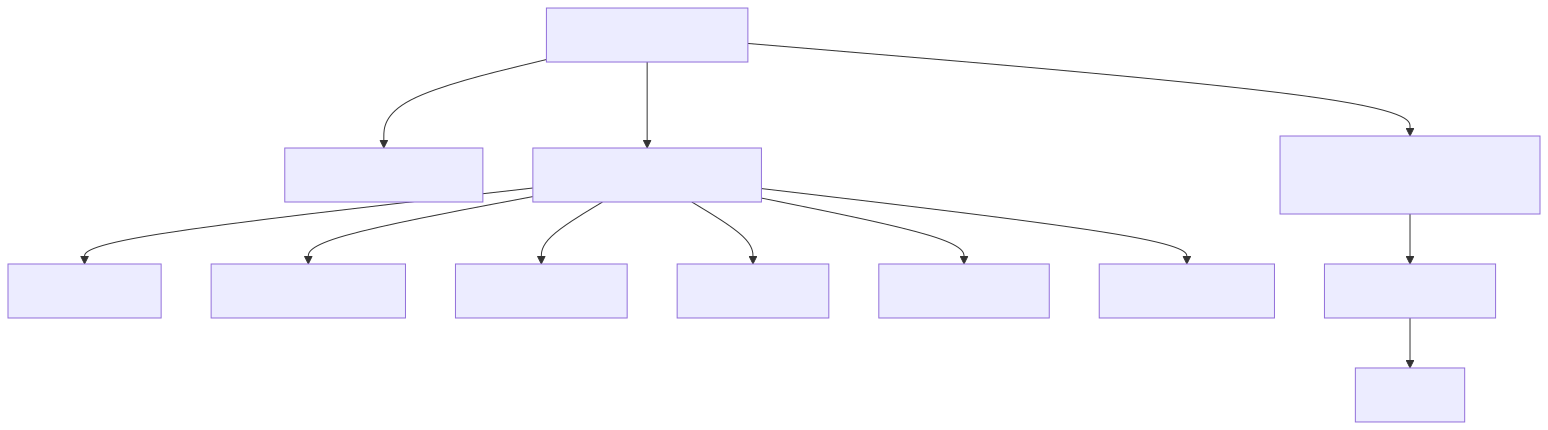
\includegraphics[width=\textwidth]{png_files/main_py_architecture.png}
\caption{Architecture diagram of \texttt{main.py} showing entry point, initialization of components, and connections to the UI.}
\end{figure}

\noindent
\textbf{Explanation:} \\
\texttt{main.py} is the application's entry point, responsible for initializing the backend (including file management and Git integration), setting up the Qt application and QML engine, and exposing Python backend objects to the QML frontend. It manages the connection between the UI and backend logic, ensuring that user actions in the interface are handled by the appropriate Python classes.

\subsection{Main.qml}

\begin{figure}[h]
    \centering
    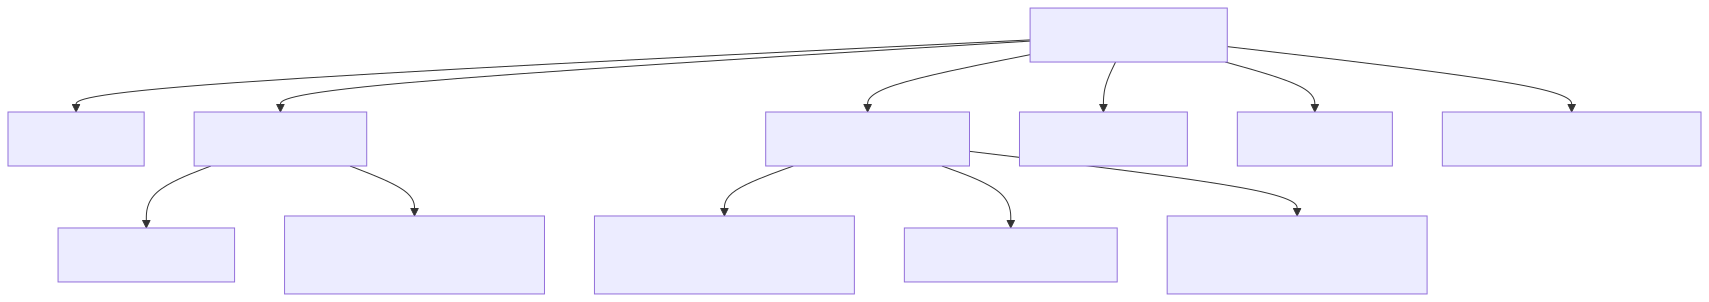
\includegraphics[width=\textwidth]{png_files/main_qml_architecture.png}
    \caption{Diagram of \texttt{Main.qml} structure, including application window, pages, navigation, and backend context properties.}
\end{figure}

\noindent
\textbf{Explanation:} \\
\texttt{Main.qml} defines the main user interface using QML. It structures the application window, navigation, and all major pages (login, dashboard, project details, event log, settings). The UI is dynamic, responding to backend signals and exposing user actions to Python logic via context properties. The dashboard and project details pages are modular, supporting tabbed navigation and dialogs for project and team management.

\subsection{reset\_users.py}

\begin{figure}[h]
    \centering
    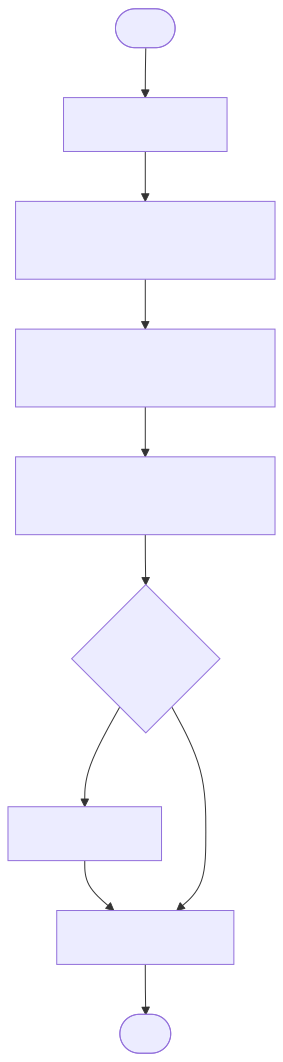
\includegraphics[width=\textwidth,height=0.8\textheight,keepaspectratio]{png_files/reset_users_flow.png}
    \caption{Diagram of \texttt{reset\_users.py} showing its interaction with the user and role tables.}
\end{figure}

\noindent
\textbf{Explanation:} \\
\texttt{reset\_users.py} is a utility script for database maintenance. It resets the user table to a predefined set of users, updating passwords and roles as needed. This ensures a consistent user base for development or testing, removing any extraneous users and enforcing correct role assignments.

\subsection{print\_users.py}

\begin{figure}[h]
    \centering
    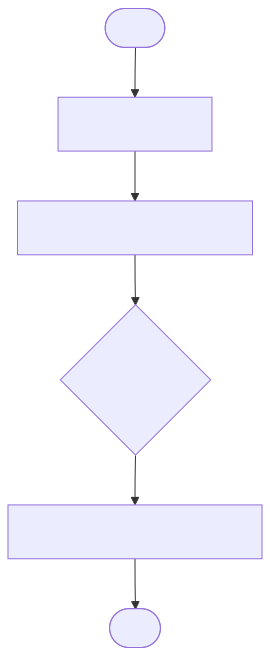
\includegraphics[width=\textwidth,height=0.8\textheight,keepaspectratio]{png_files/print_users_flow.png}
    \caption{Diagram of \texttt{print\_users.py} showing query flow for retrieving user IDs and usernames.}
\end{figure}

\noindent
\textbf{Explanation:} \\
\texttt{print\_users.py} is a simple script that queries all users from the database and prints their IDs and usernames. It is primarily used for debugging or verifying the current state of the user table.

\subsection{backend/db.py}

\begin{figure}[h]
    \centering
    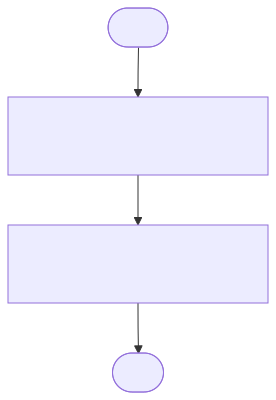
\includegraphics[width=\textwidth]{png_files/db_module_flow.png}
    \caption{Diagram of \texttt{backend/db.py} acting as a bridge to the main application database functions.}
\end{figure}

\noindent
\textbf{Explanation:} \\
\texttt{backend/db.py} acts as a bridge, re-exporting database functions and models from the main application database module. This allows backend logic to be organized and accessed consistently, supporting modularity and maintainability.



This document provides a high-level architectural overview of the main application components. Each section includes a diagram and an explanation of the component's role and structure.
\chapter{User Stories}
\section{Authentication}

- As a user, I want to log in securely, so that I can access my personalized dashboard and data.
- As an admin, I want to reset the user database, so that I can ensure only authorized users have access.

\section{Project Management}
- As a user, I want to create new projects, so that I can organize my work and tasks efficiently.

- As a user, I want to view a list of all my projects, so that I can quickly access and manage them.

- As a user, I want to edit project details such as title, description, and deadline, so that project information stays up to date.

- As a user, I want to delete projects, so that I can remove obsolete or completed projects from my workspace.

\section{Team and Role Management}
- As a project owner, I want to add team members to a project and assign roles, so that I can collaborate with others.

- As a project owner, I want to remove team members, so that I can manage project access and responsibilities.

- As a project owner, I want to assign or change the project leader, so that leadership can be transferred as needed.

- As a team member, I want to view the list of project members and their roles, so that I know who is involved.

\section{Task and Subtask Management}
- As a user, I want to add tasks and subtasks to projects, so that I can break down work into manageable pieces.

- As a user, I want to assign tasks and subtasks to team members, so that responsibilities are clear.

- As a user, I want to edit and delete tasks and subtasks, so that I can keep project plans accurate.

- As a user, I want to set deadlines, durations, and dependencies for tasks and subtasks, so that project timelines are well-defined.

- As a user, I want to categorize tasks and subtasks using the Eisenhower matrix, so that I can prioritize my work effectively.
- As a user, I want to drag and drop tasks/subtasks between categories, so that I can easily update priorities.

\section{Visualization and Planning}
- As a user, I want to view my tasks and subtasks in a dashboard, so that I can see what needs to be done today.

- As a user, I want to see a Gantt chart of project tasks and subtasks, so that I can visualize timelines and dependencies.

- As a user, I want to view a calendar with deadlines, public holidays, and personal time off, so that I can plan my work schedule.

\section{Event Logging}
- As a user, I want to see an event log of actions taken in the system, so that I can track project history and changes.

- As a user, I want to log significant actions (e.g., login, project changes, team updates), so that there is an audit trail.

\section{AI/LLM Integration}
- As a user, I want to receive AI-powered suggestions for task categorization, so that I can prioritize tasks more effectively.

- As a user, I want the system to generate commit summaries for project file changes using an LLM, so that version control messages are meaningful.

- As a user, I want to interact with local LLMs (TinyLlama, DeepSeek) for planning and suggestions, so that I can leverage AI capabilities offline.

\section{Miscellaneous}
- As a user, I want to manage my personal settings, so that I can customize my experience.

- As a user, I want to log out securely, so that my account remains protected.

\chapter{Screenshots and Interface Designs}
\chapter{Test Logs and Scripts}


\end{document}
